\chapter[Avaliação da Ferramenta]{Avaliação da Ferramenta}
\label{cap:cap4}

Nesse capítulo são apresentadas a metodologia utilizada para avaliação de usabilidade da ferramenta e-TAPE, assim como a a análise dos resultados obtidos.

% 1a seção do capítulo 4
\section{Cenário da Avaliação}
\label{sec:cenario}
O objetivo desta avaliação foi analisar a usabilidade da ferramenta desenvolvida com a utilização por possíveis usuários finais. Essa avaliação foi dividida em três etapas,
sendo a primeira a identificação do perfil dos participantes e apresentação do experimento, a segunda etapa consistem na realização das tarefas pré-determinadas, 
e por último a avaliação da usabilidade da ferramenta.

\par
Na primeira etapa, os participantes foram informados quanto ao objetivo do experimento, orientados sobre os procedimentos a serem seguidos. 
A coleta de dados sobre o perfil foi realizada através de um questionário, descrito na tabela \ref{tab:questionario}. 
O questionário original aplicado aos participantes pode ser encontrado no Anexo \ref{anexo:questionario}.

\begin{table}[!ht]
    \centering
    \caption{Dados coletados  sobre o perfil dos participantes}
    \label{tab:questionario}
    \begin{tabular}{l*{2}{>{\raggedright\arraybackslash}p{0.2\linewidth}}}
    \toprule
        Pergunta        \\
    \midrule
        Qual seu sexo? \\
        Qual sua idade?\\
        Qual seu grau de escolaridade?\\
        Você conhece o conceito de participação eletrônica?\\
        Se respondeu sim na pergunta anterior,\\ por onde conheceu o conceito de participação eletrônica?\\
        Você costuma discutir questões sociais na internet?\\
        Se respondeu sim na pergunta anterior,\\ costuma discutir com: \\
        Caso você discuta questões sociais na internet, qual(is) ferramentas utiliza? \\
        Você sabe o que é uma Taxonomia?\\
    \bottomrule
    \end{tabular}
\end{table}

\par
Após a primeira etapa, foi disponibilizada uma máquina com acesso a internet para que os participantes pudessem acessar a e-TAPE. Foi dado a cada usuário o tempo de cinco minutos para se informar sobre a TAPE, lendo as definições dos grupos, classes e subclasses,
disponíveis na primeira página da aplicação. 
Após os cinco minutos, foi entregue a cada usuário duas descrições textuais sobre ferramentas de participação eletrônica. Essas descrições foram elaboradas pelos pesquisadores envolvidos na construção da TAPE que são especialistas em participação eletrônica. 
A partir dessas descrições, cada usuário deveria classificar a ferramenta descrita usando a e-TAPE de acordo com o que achasse mais adequado.
Essa abordagem foi adotada para que fosse possível a comparação entre a classificação de uma ferramenta de participação feita por um especialista em comparação com a classificação por usuários leigos. O tempo gasto para leitura das descrições textuais e classificação das ferramentas foi cronometrado e registrado.
As descrições de ferramentas apresentadas aos participantes estão disponíveis no Apêndice X deste trabalho.

\par
Na terceira etapa, após finalizada a interação do usuário participante com a ferramenta, o objetivo foi avaliar a usabilidade da ferramenta e-TAPE.
Para essa avaliação, foi utilizado o questionário \acrfull{sus}, desenvolvido por \citeonline{brooke1996sus}, composto de 10 itens \textit{likert}. 
Cada item é associado a uma escala \textit{likert} de 5 pontos, sendo o valor 1 atribuído ao discordo totalmente e o  5 atribuído ao concordo totalmente.
A figura \ref{fig:exemplo-pergunta} exemplifica um item \textit{likert}.

\begin{figure}[!ht]
    \centering
    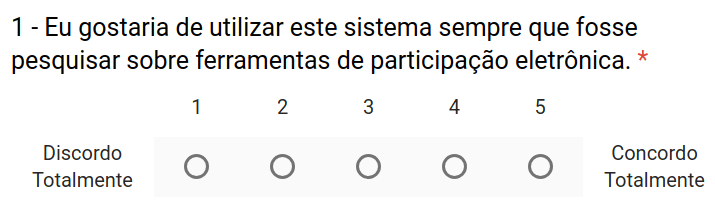
\includegraphics[scale=0.5]{./figuras/exemplo_pergunta.png}
    \caption{Exemplo de um item \textit{Likert}}
    \label{fig:exemplo-pergunta}
\end{figure}

\par
Seguindo a metodologia utilizada por \citeonline{brooke1996sus}, foi solicitado aos participantes que respondessem ao questionário, todos os 10 itens devem ser respondidos,
caso o participante não saiba como responder a algum item em especial, deve-se solicitar que responda-o com o valor três, ao centro da escala. A coleta das respostas, 
deve ser feita imediatamente ao término da leitura de cada item, evitando que se pense muito tempo sobre cada resposta, o autor alega que essa metodologia é robusta e confiável.

\par
As 10 questões que compõem o questionário foram definidas por \citeonline{brooke1996sus}, após a aplicação de um questionário sobre dois sistemas diferentes com 50 itens em potencial. Desses 50 itens, foram selecionados os 5 com os maiores valores de concordância e os outros 5 com maiores valores de discordância. Os 10 itens selecionados
foram postos alternadamente, com o objetivo de evitar respostas automáticas, obrigando o respondente a se esforçar para pensar se concorda ou discorda de cada item. 

\par
O questionário \acrshort{sus} permite o cálculo de um indicador para a usabilidade geral do sistema avaliado, denominado \textit{Score SUS} . 
\citeonline{brooke1996sus} definiu o cálculo do \textit{Score SUS} da seguinte forma:
Para os itens 1, 3, 5, 7 e 9, será o valor assinalado pelo respondente menos 1. Para os itens 2, 4, 6, 8 e 10, será 5 menos o valor assinalado. Após isso, a soma dos valores 
encontrados é multiplicada por 2,5, obtendo-se o \textit{Score SUS} para o sistema avaliado.

\par
O questionário proposto no trabalho original está descrito no Anexo \ref{anexo:questionario} e  foi adaptado ao contexto de utilização da e-TAPE de maneira que as especificidades desse domínio fossem consideradas na avaliação. O questionário utilizado está descrito na Tabela \ref{tab:questionario3}

\begin{table}[!ht]
    \centering
    \caption{Questionário SUS adaptado para avaliação da e-TAPE}
    \label{tab:questionario3}
    \begin{tabular}{l*{2}{>{\raggedright\arraybackslash}p{0.66\linewidth}}}
    \toprule
    Nº & Questão        \\
    \midrule
    1 & Eu gostaria de utilizar este sistema sempre que fosse pesquisar sobre ferramentas de participação eletrônica.\\
    2 & Eu achei a aplicação desnecessariamente complexa. \\
    3 & Eu achei a aplicação fácil de usar.\\
    4 & Eu acho que precisaria de apoio de um suporte técnico para ser possível interagir com essa aplicação.\\
    5 & Eu achei que as diversas funções nesta aplicação foram bem integradas. \\
    6 & Eu achei que houve muita inconsistência ou erros nesta aplicação. \\
    7 & Eu imaginaria que a maioria das pessoas, interessadas em ferramentas de participação eletrônica, aprenderia a usar essa aplicação rapidamente. \\
    8 & Eu achei a aplicação muito complicada. \\
    9 & Eu me senti muito confiante quanto às interações com essa aplicação. \\
    10 & Eu precisei aprender muitas coisas sobre ferramentas de participação eletrônica para que eu pudesse fazer uso da aplicação.\\
    \bottomrule
    \end{tabular}
\end{table}


\par
\citeonline{boucinha2013avaliaccao} afirmam que as questões do \acrshort{sus} podem ser associadas aos componentes de qualidade descritos por \citeonline{nielsen199510},
da seguinte forma:

\begin{table}[!ht]
    \centering
    \caption{Componentes de qualidade de \citeonline{nielsen199510} x Questões \acrshort{sus}}
    \label{tab:componentesQualidadePorQuestao}
    \begin{tabular}{l*{2}{>{\raggedright\arraybackslash}p{0.2\linewidth}}}
    \toprule
        Componente de Qualidade & Questão(ões)        \\
    \midrule
        Facilidade de aprendizagem & 3, 4, 7 e 10 \\
        Eficiência & 5, 6 e 8 \\
        Facilidade de memorização & 2 \\
        Minimização dos erros & 6 \\
        Satisfação & 1, 4 e 9\\
    \bottomrule
    \end{tabular}
\end{table}

\par 
De acordo com os autores, para avaliar cada componente de qualidade, deve-se fazer a média dos valores encontrados durante o cálculo do \textit{Score SUS} para o grupo de perguntas 
em questão \cite{nielsen199510}. Os resultados encontrados foram analisado e estão descritos na Seção \ref{sec:resultados}. 

\section{Resultados}
\label{sec:resultados}

Participaram 12 voluntários no experimento, sendo 75\% do sexo masculino e 25\% do sexo feminino, como apresentado no gráfico da Figura \ref{fig:grafico-sexo}. Além disso, 
é possível observar, pela Figura \ref{fig:grafico-idade}, que a maioria dos participantes tem entre 21 e 25 anos de idade e 
estão com a graduação atualmente em curso, como representado na Figura \ref{fig:grafico-grau}.

\begin{figure}[!ht]
    \centering
    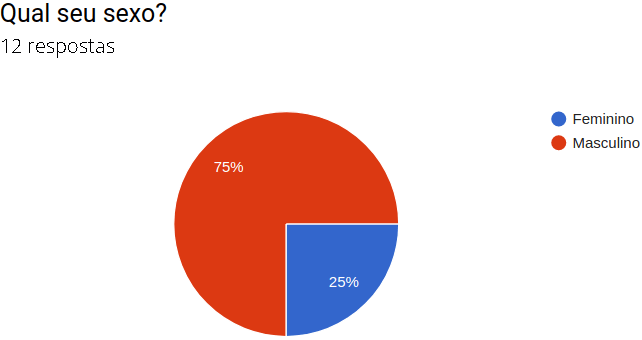
\includegraphics[scale=0.4]{./figuras/sexo.png}
    \caption{Sexo dos participantes}
    \label{fig:grafico-sexo}
\end{figure}

\begin{figure}[!ht]
    \centering
    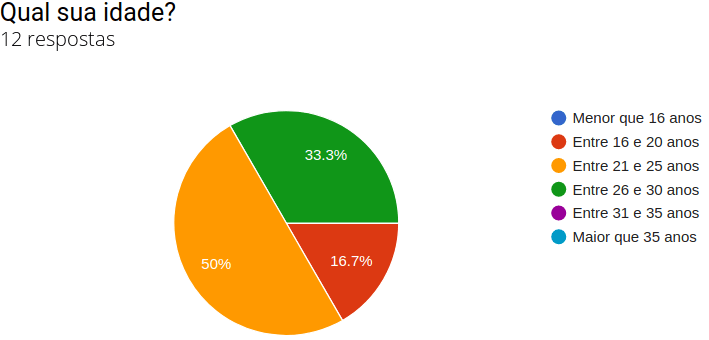
\includegraphics[scale=0.4]{./figuras/idade.png}
    \caption{Idade dos participantes}
    \label{fig:grafico-idade}
\end{figure}

\begin{figure}[!ht]
    \centering
    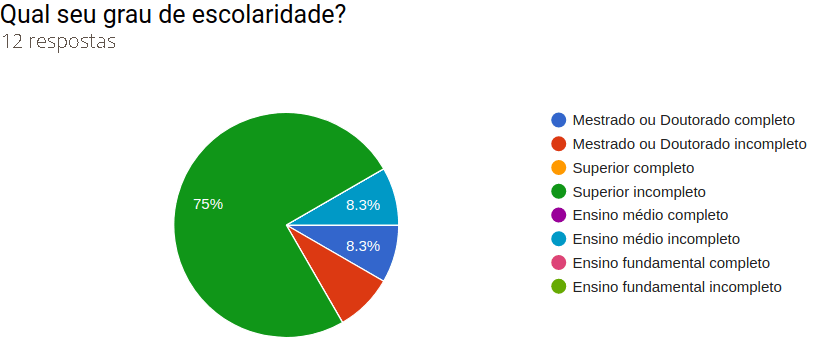
\includegraphics[scale=0.4]{./figuras/grau_escolaridade.png}
    \caption{Grau de escolaridade dos participantes}
    \label{fig:grafico-grau}
\end{figure}

\par
Pôde-se perceber que a maioria dos participantes, 91,7\%, não conhecia o conceito de participação eletrônica, resultado descrito na Figura \ref{fig:grafico-participacao}.

\begin{figure}[!ht]
    \centering
    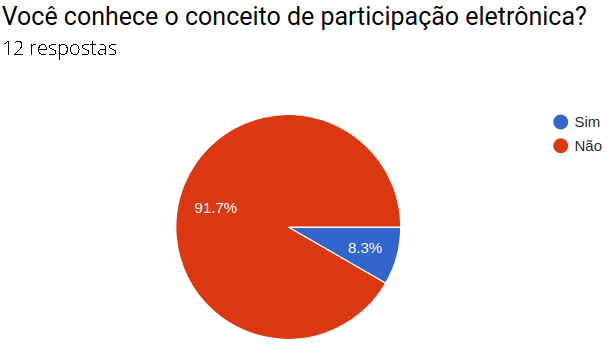
\includegraphics[scale=0.4]{./figuras/conhece_participacao_eletronica.png}
    \caption{Conhecimento sobre o conceito de participação eletrônica dos participantes}
    \label{fig:grafico-participacao}
\end{figure}

\par
Contudo, 58,3\% dos participantes, como observado na Figura \ref{fig:grafico-discu-alvo}, responderam que costumam discutir questões sociais na internet. 
Desses, 80,0\% disseram que  discutem com amigos, colegas ou conhecidos, 20,0\% discutem com amigos, colegas ou conhecidos e desconhecidos, representados pela legenda ambos
no gráfico da figura \ref{fig:grafico-discu-alvo}, ninguém respondeu que discute apenas com desconhecidos. Quando perguntados sobre quais ferramentas de participação 
eletrônica eles utilizam para discutir esse tipo de questão, 100\% das respostas foram redes sociais. 

\begin{figure}[!ht]
    \centering
    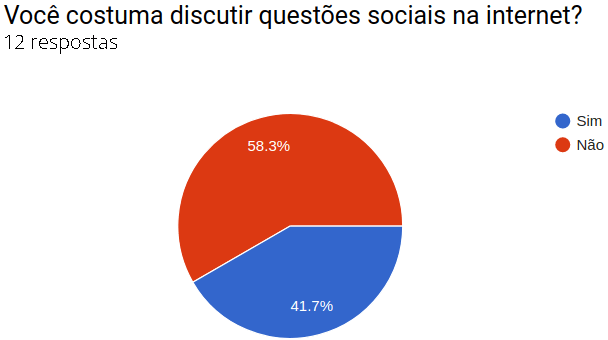
\includegraphics[scale=0.4]{./figuras/discutir.png}
    \caption{Participantes que discutem questões sociais na internet}
    \label{fig:grafico-discu}
\end{figure}

\par
Esse resultado sugere que a discussão sobre questões sociais é importante para os respondentes. Essa característica dos participantes pode ser um indicativo de que a amostra 
considerada tem uma afinidade com o tema investigado uma vez que as ferramentas classificadas estão inseridas nesse universo da participação sendo mediada pelas \acrshort{tic}. 

\begin{figure}[!ht]
    \centering
    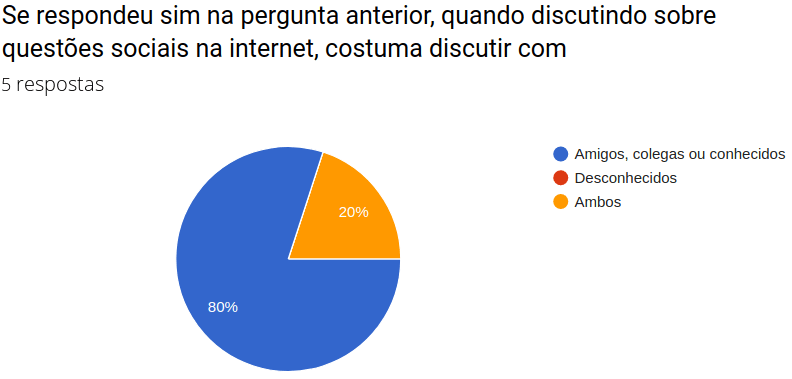
\includegraphics[scale=0.4]{./figuras/discutir_com.png}
    \caption{Pessoas com as quais os participantes que discutem questões sociais na internet interagem.}
    \label{fig:grafico-discu-alvo}
\end{figure}

\par
Quanto a última pergunta da primeira etapa, sobre o conhecimento do conceito de Taxonomia, percebeu-se que a grande maioria, 83,3\% não conhecia esse conceito conforme ilustrado na 
Figura \ref{fig:grafico-conhe-taxonomia}. Esse resultado pode ser um indicativo que mesmo a taxonomia sendo um modelo de classificação antigo, 
não faz parte do escopo de conhecimentos gerais de algumas pessoas.

\begin{figure}[!ht]
    \centering
    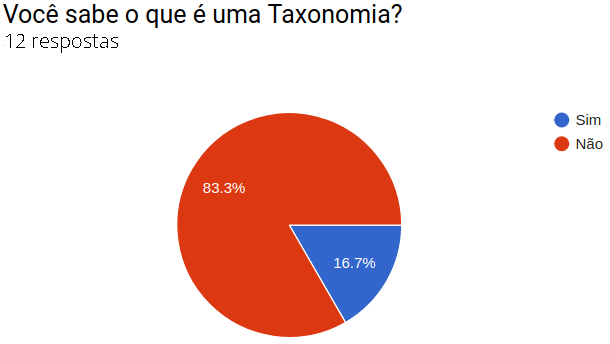
\includegraphics[scale=0.4]{./figuras/sabe_taxonomia.png}
    \caption{Conhecimento do conceito de taxonomia pelos participantes.}
    \label{fig:grafico-conhe-taxonomia}
\end{figure}

\par
O tempo médio dos participantes para a conclusão da classificação das duas ferramentas solicitadas foi de 24 minutos e 16 segundos, o gráfico na Figura \label{fig:grafico-tempo}
representa o tempo gasto por cada participante. Notou-se que participantes que tinham conhecimento prévio sobre ferramentas de participação realizaram 
as tarefas em um tempo 50\% menor se comparado aqueles que não tinham esse tipo de conhecimento.

\par 
O \textit{Score SUS} da aplicação e-TAPE foi de 78,75\%. A Tabela \ref{tab:resultado-questionario} apresenta a média de pontuação de cada item do questionário \acrshort{sus}.

\begin{table}[!ht]
    \centering
    \caption{\textit{Score SUS} de cada item do questionário aplicado}
    \label{tab:resultado-questionario}
    \begin{tabular}{l*{3}{>{\raggedright\arraybackslash}p{0.66\linewidth}p{0.1\linewidth}}}
    \toprule
    Nº & Questão & \textit{Score}    \\
    \midrule
    1 & Eu gostaria de utilizar este sistema sempre que fosse pesquisar sobre ferramentas de participação eletrônica. & ::X \\
    2 & Eu achei a aplicação desnecessariamente complexa. & ::X \\
    3 & Eu achei a aplicação fácil de usar. & ::X \\
    4 & Eu acho que precisaria de apoio de um suporte técnico para ser possível interagir com essa aplicação. & ::X \\
    5 & Eu achei que as diversas funções nesta aplicação foram bem integradas.  & ::X \\
    6 & Eu achei que houve muita inconsistência ou erros nesta aplicação.  & ::X \\
    7 & Eu imaginaria que a maioria das pessoas, interessadas em ferramentas de participação eletrônica, aprenderia a usar essa aplicação rapidamente. & ::X \\
    8 & Eu achei a aplicação muito complicada.  & ::X \\
    9 & Eu me senti muito confiante quanto às interações com essa aplicação.  & ::X \\
    10 & Eu precisei aprender muitas coisas sobre ferramentas de participação eletrônica para que eu pudesse fazer uso da aplicação. & ::X \\
    \bottomrule
    \end{tabular}
\end{table}

\par
A Tabela \ref{tab:resultado-componentes} apresenta o resultado dos componentes de qualidade do \textit{software}. Sendo assim possível chegar a conclusão, pela metodologia aplicada, 
que a ferramenta e-TAPE satisfaz os critérios de qualidade propostos por \citeonline{nielsen199510}, de facilidade de aprendizagem, eficiência, facilidade de memorização,
minimização dos erros e satisfação.

\begin{table}[!ht]
    \centering
    \caption{Valor encontrado para cada componente de avaliação da qualidade da ferramenta e-TAPE}
    \label{tab:resultado-componentes}
    \begin{tabular}{l*{2}{>{\raggedright\arraybackslash}p{0.1\linewidth}}}
        \toprule
            Componente de Qualidade & Valor         \\
        \midrule
            Facilidade de aprendizagem & ::X \\
            Eficiência & ::X \\
            Facilidade de memorização & ::X \\
            Minimização dos erros & ::X \\
            Satisfação & ::X\\
        \bottomrule
        \end{tabular}
\end{table}